\appendix
\begin{landscape}
	\chapter{Assessment sheet}\label{app:score}
	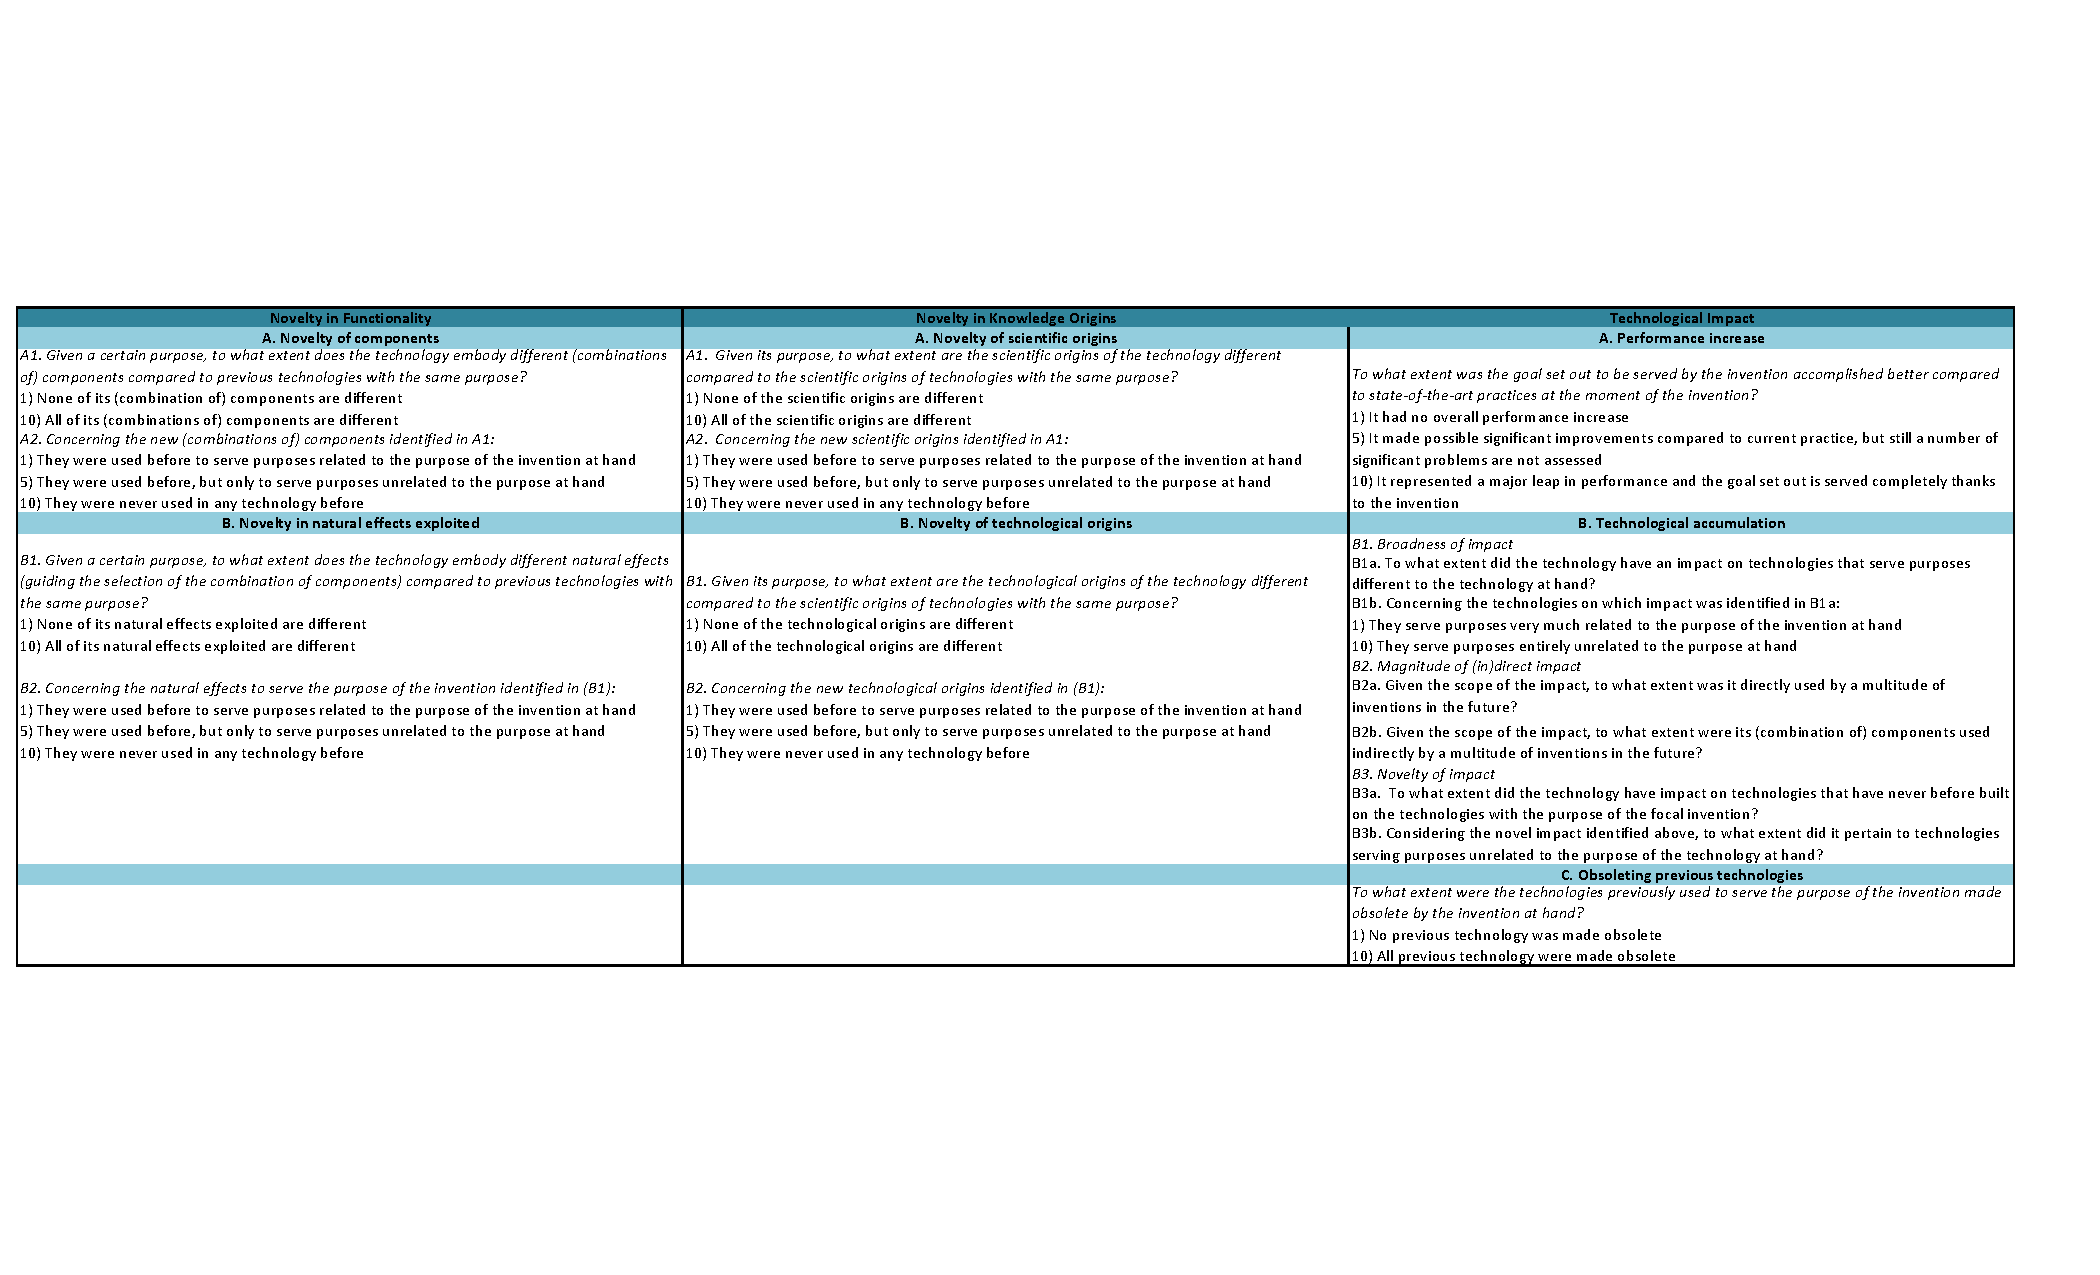
\includegraphics[width=1.0\linewidth, trim=5 150 60 150]{img/score.pdf}
\end{landscape}

\chapter{International Patent Classification codes}
This section contains a list of relevant patent categories in relation to
diagnostic medical imaging. The categories are identified using their
International Patent Classification (IPC) codes. A complete reference of all IPC
codes can be found at \url{http://web2.wipo.int/ipcpub}.

\begin{description}
  \item[A61B 1/005] Flexible endoscopes
  \item[A61B 5/05] Measuring for diagnosis by means of electric currents or magnetic fields
  \item[A61B 6/00] Apparatus for radiation diagnosis, e.g. combined with radiation therapy equipment
  \item[A61B 6/03] Computerised tomographs
  \item[A61B 8/00] Diagnosis using ultrasonic, sonic or infrasonic waves
  \item[G01N 23/00] Investigating or analysing materials by the use of wave or particle radiation
  \item[G01R 33/00] Arrangements or instruments for measuring magnetic variables
  \item[G01T 1/36] Measuring spectral distribution of X-rays or of nuclear radiation
  \item[G01T 1/161] Applications in the field of nuclear medicine, e.g. in vivo counting
  \item[G02B 23/24] Instruments for viewing the inside of hollow bodies, e.g. fibrescopes
  \item[G03B 42/02] using X-rays
  \item[G06T] IMAGE DATA PROCESSING OR GENERATION, IN GENERAL 
  \item[H01J 35/00] X-ray tubes
  \item[H05G] X-RAY TECHNIQUE
\end{description}